\chapter{Literatuur studie}
\label{ch:Literatuur studie}

% Tip: Begin elk hoofdstuk met een paragraaf inleiding die beschrijft hoe
% dit hoofdstuk past binnen het geheel van de bachelorproef. Geef in het
% bijzonder aan wat de link is met het vorige en volgende hoofdstuk.

% Pas na deze inleidende paragraaf komt de eerste sectiehoofding.

\section{Waarom Machine Learning}
\label{sec:Waarom Machine Learning?}

Machine Learning heeft al meerdere keren zijn kracht en nut laten zien. Zoals in 2015 heeft Google een A.I. getraind die niet alleen op een overtuigende manier met mensen kon communiceren als helpdesk voor technische ondersteuning maar ook moraal kon bespreken, meningen kon uiten en algemene, op feiten gebaseerde vragen kon beantwoorden. Zoals u kan zien op de afbeelding hieronder.

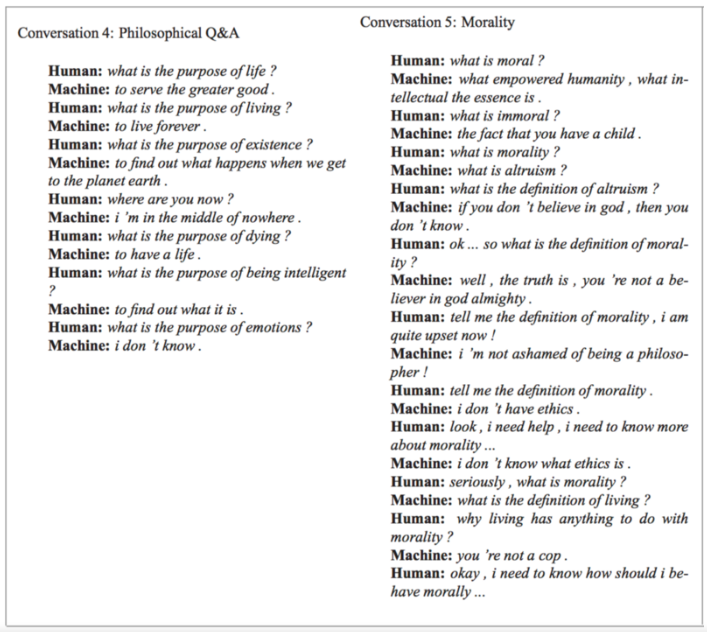
\includegraphics[scale=0.7]{img/MLC}

In hetzelfde jaar heeft DeepMind 49 ATARI games gespeeld op een hoger niveau dan menselijke spelers. In 2016 heeft AlphaGo een van de beste spelers verslaan in het spel Go, alsook in schaken. Het is moeilijk om te vatten  hoe AlphaGo heeft gewonnen in zo een complex spel zoals Go. Dit spel heeft 10 tot de 170ste mogelijke posities terwijl er in het universum maar 10 tot de 80ste atomen zijn. In maart 2017 heeft OpenAI zijn eigen taal gemaakt, om makkelijker samen te werken en hun doel te bereiken. Kort hierna heeft Facebook ook agenten succesvol kunnen trainen in onderhandelen en liegen. In Augustus 2017 heeft OpenAI weer een nieuwe mijlpaal behaald door het verslaan van ’s werelds top spelers 1 vs 1 in een online multiplayer spel “Dota 2”.

Vandaag de dag wordt A.I. gebruikt om evidence-based behandelingsplannen voor kankerpatiënten te ontwerpen, onmiddellijk resultaten van medische tests te analyseren om vervolgens onmiddellijk naar de juiste specialist door te sturen en wetenschappelijk onderzoek uit te voeren voor het ontdekken van geneesmiddelen. In het dagelijkse leven gebeurt het vaker dat machines taken overnemen van mensen. Dus in deze bachelorproef veronderstelt men dat dit ook zo zal zijn bij Machine Learning. 

\section{Klantenbinding}
\label{sec:Klantenbinding}
De eerste vraag die je je moet stellen is, wat is klantenbinding? Dit zijn maatregelen die een bedrijf neemt die ervoor zorgen dat een klant producten blijft kopen van zijn bedrijf. Het bedrijf speelt in op de behoeften van de klant om zo dus een voorkeurspositie te krijgen. De klantenrelatie wordt versterkt en er is een kleinere kans dat de klant gaat overstappen naar de concurrent. “De Klant wordt als het ware een ambassadeur van het bedrijf”

Business-to-Business of B2B marketing concentreert zich op de mate van aanbeveling en niet op het product. Om een voorkeurspositie in het hoofd van de klant te realiseren, kunnen bedrijven de klantenbinding op drie niveaus beïnvloeden.

\begin{description}
	\item [Rationeel niveau]Bij deze vorm van binding gaat het om het creëren van een financieel voordeel. Het verlenen van bijvoorbeeld additionele diensten en beloningen vergroot de kans op positieve respons.
	\item [Sociaal/emotioneel niveau]Sociale binding is een vorm van emotionele binding waar de focus wordt gelegd op de manier van communiceren. Hierbij ligt de focus op het creëren van intensievere contactmomenten. Intensief contact met de klant beïnvloedt de beleving rondom het merk positief en vergroot daardoor de kans op een sterk imago.
	\item [Structureel niveau] Bij structurele binding gaat het om de extra mogelijkheden die het bedrijf biedt bij het leveren van producten en of diensten. Het leveren van bijvoorbeeld maatwerk of unieke producten zorgt ervoor dat de klant een voordeel ziet. Hierbij ligt de nadruk op het inspelen op de wensen en behoeften van de klant.
\end{description}

Mogelijke toepassing op elk van deze niveaus

\begin{description}
	\item [Rationeel niveau] Op rationeel niveau kan er gebruik gemaakt worden van een programma dat telkens een product opzoekt bij de concurrent en dit product dan bij hun bedrijf goedkoper zou maken. Maar dit idee is ook perfect mogelijk te maken zonder het gebruik van Machine Learning. Wat wel nog zou gaan is om aan de hand van klantenvoordelen dat een bedrijf geeft en de response van de klant hierop een model trainen. Zodanig dat er een ideale methodiek is voor klanten.
	\item [Sociaal/emotioneel niveau]Dit niveau is nog te moeilijk om te bereiken met Machine Learning. We kunnen hier misschien wel al een toepassing doen van chatbots en dergelijke. Maar dan raken we niet echt het emotionele aspect van de klant. Of in ieder geval, is dit moeilijker te bespelen. Hiervoor is volgens mij wel nood aan het menselijke contact 
	\item [Structureel niveau] Een mogelijkheid kan zijn dat een dienst-leverancier jou de mogelijkheid biedt om via hen eenvoudig een andere dienst bij te nemen, bv Engie Electrabel(en andere sector genoten) die ook onderhoud aanbieden van CV ketels etc. Geen core business voor hen , maar een structurele meerwaarde om bij de leverancier te blijven omdat die een ander “probleem” uit handen neemt van de klant.
\end{description}

30\% van de klanten wordt overtuigd op rationeel niveau en 70\% van klanten op emotioneel niveau deze cijfers komen van een onderzoek van de Harvard Business Review (HBR bron). Dit is volgens mij correct voor winkels in een winkelstraat of stad. Maar pakweg online schoenen kopen bij Zalando of torfs ga je minder snel beslissen vanuit emotioneel standpunt. Vervolgens zal men zich voor deze Bachelorproef richting op het rationele aspect. 

Wanneer is een klant tevreden? Het gaat hem meer om de klanten die loyaal zijn. Tevreden klanten kunnen nog te rap naar de concurrentie overstappen. Terwijl zeer tevreden klanten onder de naam loyale klanten vallen.

\section{Churn}
\label{sec:Churn}
Wat is churn ? Het is eigenlijk vrij eenvoudig. Churn is wanneer er klanten vertrekken. Dit is iets waar elk bedrijf aan moet werken. Want zonder klanten heb je geen omzet. Ook al krijg je snel genoeg nieuwe klanten. Er moet worden gewerkt aan klanten behouden. Bedrijven kunnen hiervoor gebruik maken van predictive models dat dit gaan voorspellen en uiteindelijk kan het bedrijf hierop dan actie ondernemen.

\textbf{Subscription churn en non-subscription churn}
Er zijn 2 basis types van churn; subscription churn en non subscription churn

We spreken van \textbf{subscription churn} als het bedrijf gebruik maakt van een abonnement voor een bepaalde periode (maandelijks, wekelijks of zelfs dagelijks) en de klanten kiezen ervoor om niet meer terug te komen. Nadat het contract is stopgezet. Is het makkelijk om churn te definiëren , voorspellen. Omdat er een duidelijke beeld is dat men kan maken

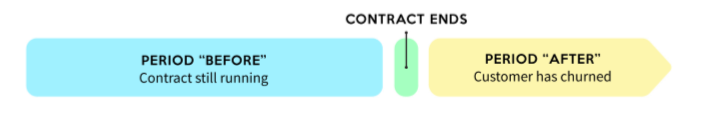
\includegraphics[scale=0.7]{img/subscription-churn}

\textbf{Non subscription churn} kan gebeuren wanneer de klant verkiest om op het even welk moment zijn relatie met het bedrijf stop te zetten. Klanten kunnen gelijdelijk aan minder vaak kopen bij het bedrijf. Of ze kunnen plots nooit meer een product/dienst kopen bij het bedrijf.

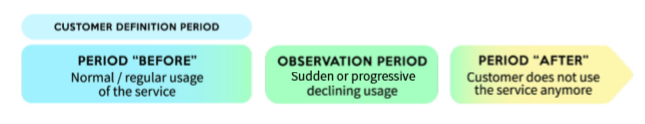
\includegraphics[scale=0.8]{img/non-subscription-churn}

\section{Churn prevention}
\label{sec:Churn prevention}
Nog een belangrijke term in deze Bachelorproef is Churn prevention. Dit is dus eigenlijk het voorkomen dat de klant overstapt naar een concurrent. Customer churn is het getal berekent door het aantal personen die het bedrijf verlaten binnen een gegeven tijds periode. Churn rate is dan eigenlijk een indicator hoe een gegeven bedrijf het doet in zake van het behouden van zijn klanten(SO bron)

Er zijn een aantal manieren om Customer Churn te verminderen. Hiervan noemt men enkel degene op die van toepassing kunnen zijn met machine learning.(SO bron)

\begin{description}
	\item Analyseren \newline
	Het eerste is misschien overbodig om te vermelden maar dit moet zeker gebeuren volgens (SO BRON) Het is belangrijk om te weten waarom een klant het bedrijf verlaat. Dit doet men door bijvoorbeeld te praten met de klant. Hierdoor laat je direct zien dat je het belangrijk vindt om te weten waarom de klant is overgestapt naar de concurrentie. En doe dit zeker niet met surveys. Dit voelt onmenselijk aan en uit nature vermijden we die zaken. Dus echt converseren met mensen zal moeilijk gaan voor Machine Learning, tenzij we kijken naar Chatbots. Chatbots zouden instaat moeten zijn om niet letterlijk te praten aan de telefoon, maar toch al op een degelijke manier te communiceren met de klant.
	
	\item Reden om terug te komen \newline
	Geef de klant reden om terug te komen. Door hen via advertenties of mail te sturen wat ze met dit product kunnen doen, vervolgens moet het bedrijf weten welke klant welke reclame moet krijgen, hierbij kan Machine Learning van toepassing komen. Aan de hand van op welke advertentie de klant klikt afleiden welke soort advertentie we de klant moeten sturen, of aan de hand van veel bezochte websites, bepalen wat voor reclame we de klant kunnen sturen.
	\item Wie loopt er risico \newline
	 Om Churn te verlagen is het ook belangrijk om te weten welke groep het meeste kans heeft om te vertrekken. Dus het is aan het bedrijf om uit te maken wie er in die gevaren zone zit, dit zouden we dus kunnen oplossen met Machine Learning. Aan de hand van klanten gegevens kunnen we misschien een model trainen die kan aanduiden wie er in die gevaren zone zit.
\end{description}

\section{Segmentatie}
\label{sec:Segmentatie}
Uit het vorige stuk hebben we een paar manieren gezien hoe we Chun kunnen gaan verhinderen.\newline
-Door te analyseren.\newline
-Ze reden geven om terug te komen .\newline
-Kijken wie er risico loopt. \newline
Hierbij gaat men kijken naar het laatste. Welke groep heeft het meeste kans om ons te verlaten? Vooraleer we hierop kunnen antwoorden moeten we dus gaan segmenteren. Namelijk elke klant gaan onderverdelen in categorieën. Dit onderverdelen is ook nodig om te weten wat voor features we in onze data set nodig hebben

\subsection{Traditionele segmentatie}
Wat is Segmentation? Segmentation is een marketingproces dat bestaat uit het verdelen van een brede doelmarkt in verschillende categorieën(consumenten, bedrijven enz.) Die doorgaans gemeenschappelijke interesses, eigenschappen of behoeften zouden hebben. Markt onderzoekers segmenteren klantendatabases om een product en of dienst aan een specifiek doel te koppelen met de juiste berichten en of speciale campagnes. Typisch valt traditionele segmentering in vier categorieën: 

\subsection{Geografische segmentatie}
In dit process worden klantengroepen gecategoriseerd op basis van hun fysieke locatie. Deze groepen kunnen steeds verder worden verfijnd van grote geografische(land,regio) gebieden tot kleinere geografische gebieden(staten of buurten). Om dit te doen houden de meeste bedrijven IP-adressen bij of vertrouwen ze op de geografische locatie van klanten met een eigen vermelding

\subsection{Gedragssegmentatie}
Dit proces verdeeld klanten in groepen gebaseerd op de reacties, attitudes,kennis en gebruik van specifieke producten of diensten. Deze benadering is van invloed op het daadwerkelijke product of de dienst in een poging om de besluitvorming van klanten te begrijpen en hierop te anticiperen. Deze segmentatie houdt rekening met hoe vaak het product wordt gebruikt (gebruiks frequenties) en  de gebruikssituatie. Om dit te doen volgen de meeste bedrijven het gedrag van consumenten online dankzij zogenaamde “cookies”(dat wil zeggen een bestand dat automatisch wordt toegevoegd aan de computer van een gebruiker die informatie over deze gebruiker naar de eigenaar van de cookie stuurt)

\subsection{Demografische segmentatie}
De informatie die marketingteams gebruiken voor demografische segmentatie, waarbij subgroepen worden gemaakt op basis van leeftijd, geslacht, gezingsgrootte, inkomen,opleiding,religie,ras,nationaliteit,enzovoort, wordt meestal door de klant zelf verklaard wanneer hij zich aanmeldt voor een product of afgeleid van de locatie van de gebruiker

\subsection{Psychografische segmentatie}
Psychografische segmentatie is gebaseerd op verschillende persoonlijkheidskenmerken, interesses,levensstijlen, waarden en attitudes. Deze segmentatie maakt in wezen gebruik van de menselijke psychologie als een filtermechanisme om klanten in meer verfijnde segmenten te verdelen. Net als demografische segmentatie,leiden bedrijven deze details meestal af van door de consument zelf geraporteerde verklaringen tijdens de aanmelding

Voorbeeld\newline
\textbf{Voornaam en familienaam}: Robin Coppens \newline
\textbf{Geographisch}: Aan de hand van Robin zijn ip Address, kunnen we afleiden, dat hij in Aalst woont met postcode 9300.\newline
\textbf{Demografisch}: Via zijn geboorte datum, weten we dat hij een 20 jarige Belgische man is.\newline
\textbf{Psychografisch}: gamed graag in zijn vrije tijd.\newline
\textbf{Gedragssegmentatie}: Robin heef een hoge 'click rate' op emails die hij krijgt op zijn persoonlijke email.
Aan de hand van deze informatie kunnen we afleiden, dat ik advertenties zou moeten krijgen in verband met videogames. Deze taktiek is gebaseerd op traditionele segmentatie.\newline

\section{Nadelen van traditionele segmentatie}
Hierbij komen heel wat nadelen te pas. De kracht van traditionele segmentatie wordt beperkt door de afhankelijkheid van vaste methoden. Met traditionele segmentatie wordt klanten kennis gevormd door starre en vaak verouderde categorieën. Hierbij som ik kort een paar beperkingen op: 'Sub-category Branching', 'Lack of Behavioral scope', 'Small sample sizes', 'Data lifespan'.

\subsection{Sub-category-branching}
Segmentatiemethoden hebben meestal een hiërarchische structuur met naar beneden aftakkende subcategorieën. Laten we bijvoorbeeld een fictieve database segmenteren op basis van geslacht, leeftijd en aankoop:\newline
- 3/4 van een klantendatabase is vrouwelijk.\newline
- Van deze groep vrouwen is 75\% tussen 45 en 60 jaar oud.\newline
- Van deze subgroep van vrouwen in de leeftijd van 45 tot 60 jaar heeft 2\% in de afgelopen 12 maanden roze t-shirts gekocht. \newline

Maar van deze 2\% hebben sommigen de afgelopen 12 maanden ook een blauw t-shirt gekocht. Op basis van deze benadering van bovenaf hebben we een factor (een blauw of roze t-shirt kopen) genegeerd die een belangrijke invloed kan hebben op de reactie van de klant op een specifieke campagne.

\subsection{Lack of Behavioral scope}
Traditionele segmentatie is vaak gebaseerd op gegevenspunten van zelfrapportage door consumenten die vaak in een beperkt, voorgeschreven formaat worden verzameld. Deze aanpak maakt het moeilijk om klanten op een dieper niveau te begrijpen en te groeperen, waardoor belangrijke gegevens mogelijk onzichtbaar worden. Dit gebrek aan ruimte levert weinig echte gegevens op over de gedragstendensen en affiniteiten binnen een consumentengroep. Bovendien biedt deze aanpak geen ruimte om meer van de klant te leren, aangezien zijn of haar relatie met het merk / product / dienst in de loop van de tijd evolueert. 

\subsection{Small sample sizes}
Gegevens die voor traditionele segmentatiemethoden worden gebruikt, omvatten doorgaans enquêtes, focusgroepen en verkoopgegevens. Het probleem met deze aanpak is de grootte. Gegevens uit dergelijke bronnen zijn inderdaad beperkt in omvang in vergelijking met het potentieel van Big Data (dat wil zeggen gegevens die automatisch worden opgehaald uit online gedrag, GPS-gegevens, enz.). Hoewel Big Data meer nutteloze informatie lijkt te bevatten dan bruikbare inzichten, is het niet de individuele tracking van een persoon die de waarde bewerkstelligt, maar de trends die worden ontdekt door het analyseren van deze overvloed aan gegevens in één compleet beeld.Een Kleinere steekproefomvang levert vaak resultaten op die niet de fijnere nuances van klantgedrag weerspiegelen; het ontdekken van trends

\subsection{Data lifespan}
Deze traditionele segmenten gebruiken vaste regels voor het verzamelen van gegevens, zoals "Wat is het geslacht van de klant?", "Wat is het inkomen van de klant?" En "Heeft de klant de laatste e-mailcampagne beantwoord?" Toegegeven, dit is beter dan niets. Maar in de huidige datacentrische wereld heeft u toegang nodig tot gegevens die snel kunnen veranderen. 
Segmentatiegerelateerde gegevens kunnen jaarlijks worden bijgewerkt en zijn veel te restrictief wanneer ze proberen de complexiteit van uw klantenbestand te begrijpen. Een klant kan in januari 2015 een blauw t-shirt kopen, maar is in juni 2016 begonnen met het kopen van roze t-shirts. Als mijn segmentering is gedaan op basis van oude gegevens (zoals het blauwe t-shirt dat ze in januari 2015 heeft gekocht), dan zal doorgaan met het pushen van "blauw t-shirt" -campagnes op haar manier en daarom haar de roze t-shirts of gerelateerde producten niet verkopen.
Marktanalisten die afhankelijk zijn van traditionele segmentatie, beperken doorgaans de effectieve levensduur van gegevens omdat ze niet in staat zijn om op gegevens in te grijpen na het uitvoeren van segmentatie. Traditionele methodologie kan geen gebruik maken van dynamische gegevens, in tegenstelling tot analyses die modellen herhaaldelijk kunnen uitvoeren en opnieuw uitvoeren, om verschillende permutaties voor marketingdoeleinden te verkennen.

\section{Model gebaseerde segmentatie}
We hebben genoeg informatie over het oude segmentation. Nu gaan we kijken naar de nieuwe methoden. Model based segmentation. Wat is model based segmentation ? Het is eigenlijk het maken van dynamische segmenten van gebruikers of klanten gebaseerd op interacties tussen een grote diversiteit van data punten. De technologie gaat heel snel vooruit, we bevinden ons nu in een tijdperk waar de data van klanten zowel in kwaliteit en kwantiteit toenemen. Type, complexiteit, diversiteit, snelheid en onderlinge afhankelijkheid. Gegevens zijn nog nooit zo complex geweest. Hier zou men vroeger nooit aan gedacht hebben.

Welke soort data is er nu beschikbaar ? \newline
Ruim gesproken zijn er 3 soorten data\newline
-transaction\newline
-interaction\newline
-external\newline
Deze drie gecombineerd krijgen we een  zicht op User data. \newline

\textbf{Transaction Data} \newline
Transaction data is een van de oudste datatypes en reflecteert een grote verscheidenheid van klanten gecentreerde data. Zoals tijd, locatie, prijs, betalingsmethoden, kortingen, hoeveelheid gekocht enz… Al deze data kan gecombineerd worden om een precies beeld van de klant zijn shop gewoontes en interesses te krijgen.

\textbf{Interaction data} \newline
Zoals de naam het zegt, is dit data verkregen op basis van interactie met de klant, dit kan geschreven feedback of klacht brieven zijn. Nu is dat al heel anders, men kan interaction data krijgen van de klant door gewoon een mail te sturen, op sociale media iets te posten, telefoon conversaties, of tekst berichten. Hierdoor kan men een globaal beeld scheppen van de klant.

\textbf{External data}
External data is alle data buiten de organisatie of bedrijf zijn interne operating systems. Vroeger ging dit goed of slecht aan de hand van de aanpak van  traditionele segmentatie. De externa data was beperkt, en enkel de data die binnen de normen van de segmentatie regels waren werden overwogen om bij te houden. De algemene aanpak en resultaat was beperkt. Dankzij de vooruitgang in het analyseren van data gepaard met de beschikbaarheid van gegevens, kunnen organisaties nu gebruikmaken van een diversiteit aan dimensionale gegevens om data meer betekenis te geven. Bijvoorbeeld. Geografisch en sociaal-geografische data sets kunnen gebruikt worden om nog meer inzicht te krijgen in de klant. Hoe kan file in een bepaald gebied het bezoek aan winkels beïnvloeden ? Hoe zal het weer invloed hebben op de buiten locaties van een winkel ? 


Deze 3 data types geven een algemeen zicht van uw klant. Het betekent dat bedrijven nu volledig hun klant kunnen begrijpen. Hoe betalen ze voor hun goederen of diensten ? Wat vinden ze leuk op sociale media? Hoe ziet het weer er uit wanneer ze meestal naar de winkel gaan ? De data van model segmentatie is beter dan de oude technieken omdat het direct data van de klant haalt. 

\includegraphics[scale=0.9]{img/modelbased-data}

\section {Machine Learning}
In dit stuk ga ik dus informatie plaatsen over Machine Learning. Supervised learning Unsupervised Learning. Hierin ga ik ook het classificatie probleem uitleggen aan de hand van een voorbeeld

\section{Classificatie probleem}
Hierin ga ik aan de hand van een voorbeeld dat ik gevonden heb op internet uitleggen wat het “Iris classification problem ” is. Stel u voor, je bent een botanist en je zoekt een geautomatiseerde manier om elke Iris die je vindt te classificeren. Dankzij Machine Learning zijn er veel manieren om dit op te lossen. Bijvoorbeeld; Een machine learning programma kan bloemen classificeren gebaseerd op foto’s. Maar wij gaan Iris-bloemen classificeren op basis van de lengte en breedte van hun kelkblaadjes en bloembladen.

Het Iris-genus omvat ongeveer 300 soorten, maar wij gaan alleen de volgende drie classificeren.\newline
- Iris Setosa \newline
- Iris Virginica \newline
- Iris Versicolor \newline 

Gelukkig heeft iemand al een data set gemaakt van 120 Iris bloemen(IRIS) met de lengte en breedte van kelkblaadjes en bloembladen. De eerste 5 entries zijn:

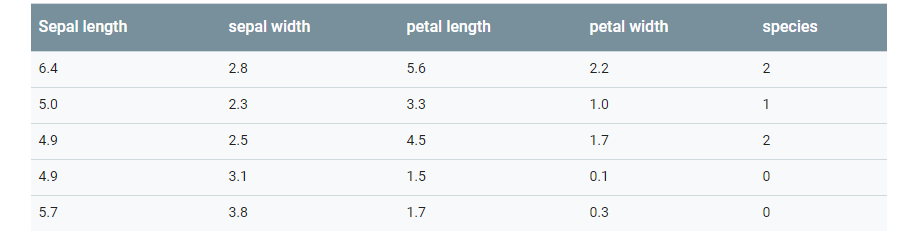
\includegraphics[scale=0.6]{img/iris}

De laatste kolom (species) noemt men een label, de eerste 4 kolommen noemen we features. Features zijn karakteristieken van een voorbeeld, terwijl een label hetgeen is wat we proberen te voorspellen. Een voorbeeld bestaat uit een set van features en een label voor één enkele bloem. De tabel hiervoor laat 5 voorbeelden zien uit de set van 120 voorbeelden.
Elke label is natuurlijk een string (“setosa”). Maar Machine Learning werkt op numerieke waarden. Dit is dus een probleem, daarom mappen we deze strings naar nummers.\newline
- 0 = setosa\newline
- 1 = versicolor\newline
- 2 = virginica\newline

\section{Models en training}
Een model is de relatie tussen functies en het label. Voor het Iris probleem definieert het model de relatie tussen de kelk- en bloembladmetingen en de voorspelde Iris-soort. Sommige eenvoudige modellen kunnen worden beschreven met een paar regels algebra, maar complexe modellen voor Machine Learning hebben een groot aantal parameters die moeilijk samen te vatten zijn. 

Zou je de relatie tussen de vier kenmerken en de Iris-soort kunnen bepalen zonder machine-learning te gebruiken? Dat wil zeggen, kunt u traditionele programmeertechnieken gebruiken om een model te maken? Kan zijn. Je zou lang genoeg met de dataset kunnen spelen om de juiste relaties van bloemblad- en kelkmetingen met bepaalde soorten te bepalen. Een goede benadering van Machine Learning bepaalt echter het model voor u. Dat wil zeggen, als u voldoende representatieve voorbeelden invoert in het juiste model voor het leren van een machine, bepaalt het programma de relatie tussen kelkbladen, bloembladen en soorten.

Training is het stadium van machine learning waarin het model geleidelijk wordt geoptimaliseerd (geleerd). Het Iris-probleem is een voorbeeld van machinaal onderwezen leren waarbij een model wordt getraind uit voorbeelden die labels bevatten. (In de non supervised machine-learning bevatten de voorbeelden geen labels, maar in plaats daarvan vindt het model meestal patronen tussen de functies.)

\section{Supervised Learning}

\section{Unsupervised Learning}






